\chapter{Analisis Persoalan dan Rancangan Solusi}

Tujuan utama penulisan bab ini adalah untuk menguraikan rencana penyelesaian masalah tugas akhir sebelum dieksekusi. Bagian ini akan memaparkan proses analisis masalah hingga menjadi solusi.

\section{Analisis Persoalan}
\label{sec:analisis-persoalan}

Berdasarkan latar belakang yang telah diuraikan pada subbab \ref{sec:latar-belakang}, peningkatan kinerja model IndoBERT dilakukan dengan menggunkan metode \textit{parameter-efficient transfer learning} (PETL). Peningkatan kinerja model dengan metode PETL ini melibatkan penambahan konfigurasi ataupun \textit{layer} tambahan terhadap model tergantung dengan karateristik dari metode PETL masing-masing. Untuk setiap metode PETL dibutuhkan \textit{dataset} tersendiri agar model dapat dilakukan \textit{transfer learning}. Selain itu, analisis komprehensif dibutuhkan untuk membandingkan metode PETL yang dapat memberikan hasil terbaik. Untuk membuat analisis yang komprehensif dibutuhkan metode evaluasi terhadap kinerja model. Secara keseluruhan, penelitian yang dilakukan pada tugas akhir ini akan mencakup tiga tahap sebagai berikut.

\begin{enumerate}
    \item Pengembangan dan konfigurasi pada setiap metode PETL.
    \item Integrasi model dengan \textit{dataset} yang dipilih.
    \item Eksperimen dan evaluasi kinerja model.
\end{enumerate}

Berdasarkan tahapan-tahapan penelitian yang diuraikan tersebut, terdapat empat persoalan utama dengan rincian sebagai berikut.

\begin{enumerate}
    \item Pemilihan \textit{dataset} yang sesuai untuk setiap tugas NLP.
    
    Berdasarkan tahap penelitian nomor 2 yaitu integrasi model dengan \textit{dataset} yang dipilih, diperlukan pencarian \textit{dataset} terlebih dahulu. Metode \textit{transfer learning} membutuhkan data yang relevan dengan tugas yang ingin dilatih. Diperlukan penilaian terhadap konten \textit{dataset} untuk memastikan kesesuaiannya dengan tugas NLP yang ditargetkan. Selain itu, kualitas \textit{dataset}, termasuk keakuratan label dan kebersihan data, serta ukurannya, harus cukup untuk memungkinkan model belajar secara efektif. Sehingga, pemilihan \textit{dataset} penting dilakukan untuk mendapatkan kinerja yang baik.

    \item Pemilihan konfigurasi terbaik untuk setiap metode PETL.
    
    Setiap metode PETL mempunyai karakteristik yang berbeda dalam penggunaannya, sehingga konfigurasi untuk setiap metode perlu diperhatikan. Proses ini melibatkan penyesuaian \textit{layer} dan parameter yang spesifik untuk setiap metode. Penting untuk mengeksplorasi berbagai konfigurasi untuk menemukan kombinasi yang paling efektif. Hal ini mencakup penyesuaian ukuran \textit{layer}, jumlah parameter, dan aspek teknis lainnya yang dapat mempengaruhi kinerja model. Selain itu, metode PETL juga memerlukan penambahan \textit{adapter} seperti pada teknik \textit{tiny-attention adapter}. Bahkan, menggabungkan beberapa metode PETL juga memungkinkan, sehingga diperlukan pembuatan konfigurasi yang spesifik untuk setiap metode.


    \item Pemilihan kombinasi \textit{hyperparameter} terbaik pada proses \textit{training}.
    
    Berdasarkan tahap penelitian nomor 3 yaitu eksperimen dan evaluasi kinerja model, proses \textit{transfer learning} melibatkan proses \textit{training}. Pada proses tersebut perlu pemilihan kombinasi \textit{hyperparameter} yang optimal. \textit{Hyperparameter} seperti \textit{learning rate}, \textit{batch size}, dan jumlah \textit{epoch} berperan penting dalam menentukan kinerja model. Proses ini melibatkan eksperimen dengan berbagai kombinasi untuk menemukan setelan yang memberikan hasil terbaik. 
    
    \item Pemilihan metode evaluasi
    
    Untuk dapat melakukan analisis terhadap model diperlukan adanya metode evaluasi yang memang relevan dengan tugas NLP-nya. Metode evaluasi yang digunakan pada proses \textit{training} berupa metrik seperti akurasi, \textit{presisi}, \textit{recall}, dan F1-\textit{score}. Sedangkan, untuk analisis komprehensif yang dilakukan terakhir akan digunakan IndoLEM sebagai \textit{NLP Task Benchmarking}

\end{enumerate}

\section{Analisis dan Rancangan Solusi}

Berdasarkan analisis masalah, terdapat beberapa solusi yang dapat langsung menjawab permasalahan yang diuraikan pada Bab \ref{sec:analisis-persoalan}. Pemetaan analisis dan rancangan solusi terhadap analisis masalah terdapat dalam tabel berikut.

\begin{table}[h!]
    \centering
    \begin{tabular}{|m{0.45\linewidth}|m{0.45\linewidth}|}
    \hline
    \rowcolor{black!10}
    \textbf{Analisis Masalah} & \textbf{Analisis dan Rancangan Solusi} \\ \hline
    (1) Kakas IndoLEM yang \textit{outdated} & (1) Refaktorisasi kakas IndoLEM \\ \hline
    (2) Pengembangan metode PETL pada kakas IndoLEM. & (2) Mengembangkan setiap metode PETL pada kakas IndoLEM \\ \hline
    (3) Pemilihan konfigurasi terbaik untuk setiap metode PETL & (3) Eksperimen terhadap berbagai konfigurasi metode PETL \\ \hline
    (4) Pemilihan kombinasi \textit{hyperparameter} terbaik pada p4oses \textit{training} & (3) Penelusuran kombinasi \textit{hyperparameter} terbaik\\ \hline
    (5) Pemilihan metode evaluasi & (4) Penelusuran metode evaluas5 yang relevan \\ \hline
    \end{tabular}
\caption{Pemetaan analisis dan rancangan solusi terhadap analisis masalah}
\label{table:pemetaan-masalah-solusi}
\end{table}

Berdasarkan analisis solusi terhadap setiap analisis masalah yang terdapat pada tabel \ref{table:pemetaan-masalah-solusi}, dibangun sebuah rancangan solusi berupa skenario pengujian yang dilakukan dalam penelitian tugas akhir, yang dapat dilihat pada Gambar \ref{fig:rancangan-solusi}.

\begin{figure}[ht]
    \centering
    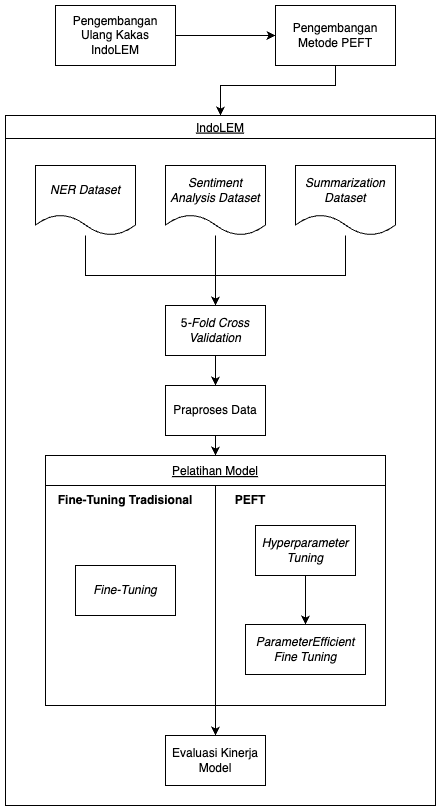
\includegraphics[width=1\textwidth]{chapter-3/rancangan_solusi.png}
    \caption{Rancangan Solusi}
    \label{fig:rancangan-solusi}
\end{figure}

Teknik PETL yang digunakan adalah LoRA (\textit{Low-Rank Adaptation}), \textit{Prefix-Tuning}, dan \textit{Tiny-Attention Adapter}. Hasil pengujian berupa kinerja dari teknik PETL serta penggunaan sumber daya dari setiap eksperimen.
\subsection{Pengembangan Ulang Kakas IndoLEM}

Pengembangan ulang ini diperlukan untuk memperbarui dan memperbaiki infrastuktur dari kakas IndoLEM. Selain itu, proses ini juga diperlukan untuk mengembangkan metode PEFT karena metode tersebut banyak memerlukan versi yang lebih baru dari pustaka yang digunakan. Untuk melakukan faktorisasi teradapat beberapa langkah yaitu memperbarui versi dari perangkat lunak, penyederhanaan dan standardisasi proses, dan dokumentasi.

Peningkatan versi Python ke versi terbaru yang kompatibel dengan pustaka yang digunakan beserta dependensinya, salah satunya adalah Torch dan Transformers. Versi pustaka yang digunakan pada IndoLEM banyak yang tidak bisa digunakan pada versi Python yang lebih baru, sehingga eksperimen sulit untuk dibuat ulang pada perangkat yang berbeda. 

\textit{Script} yang saat ini terdapat pada IndoLEM menggunakan pustaka versi lama terutama pada proses \textit{training}-nya. Sedangkan, untuk mengintegrasi metode PEFT perlu menggunakan pustaka dengan versi yang terkini. Sehingga, perlu pengembangan ulang terhadap kakas IndoLEM agar setiap prosesnya menggunakan metode dan versi yang lebih baru dari pustakanya. Selain itu, \textit{script} yang dikembangkan dari awal bisa di-\textit{reuse} terhadap setiap \textit{task}-nya untuk meningkatkan \textit{readibility} dari kodenya.

Dokumentasi pada kakas IndoLEM saat ini cukup terbatas, terutama pada \textit{requirement} untuk versi Python dan pustaka yang digunakannya, sehingga sulit untuk menajalankan eksperimennya. Perlu dilakukan dokumentasi yang lengkap terutama pada versi dari semua kakas yang digunakan pada eksperimen.

\subsection{Integrasi Metode PETL pada Kakas IndoLEM}

Proses ini bertujuan untuk mengintegrasikan metode PETL yaitu \methodPETL pada arsitektur IndoBERT. Implementasi metode PETL ini memungkinkan peningkatan kinerja model dengan menambahkan atau memodifikasi konfigurasi dan layer model sesuai dengan karakteristik masing-masing metode PETL. Terdapat beberapa alternatif dalam melakukan integrasi metode, seperti menggunakan pustaka OpenDelta dan Adapters. Tetapi, tidak tersedia semua metodenya.

LoRA adalah teknik yang memodifikasi bobot dari PLM  dengan menambahkan adapatasi berbasis \textit{rank} rendah pada bobot tersebut. Pada arsitektur IndoBERT, LoRA diintegrasikan dengan menambahkan adaptasi LoRA pada layer tertentu dari model IndoBERT. Sehingga, layer adaptasi ini berfungsi untuk mengatur interaksi antara bobot asli modle dengan adapatasi LoRA, dengan tujuan untuk memertahankan jumlah parameter yang efisien sambil meningkatkan model.

\textit{Prefix-Tuning} merupakan metode yang menambahkan sejumlah kecil parameter yang dapat dipelajari yaitu \textit{prefixes} ke dalam model. Pada implementasi dari \textit{Prefix-Tuning} ini akan ditambahkan \textit{prefixes} ke dalam \textit{input} dari model. Teknik ini memungkinkan model untuk menyesuaikan prediksinya berdasarkan konteks yang diberikan oleh \textit{prefixes}, dengan menambahkan parameter yang minimal. 

\textit{Bottleneck Adapter} adalah teknik yang mengintegrasikan adapter kecil ke dalam arsitektur \textit{attention} dari model untuk menyesuaikan output dari \textit{attention layers}. \textit{Adapter} memungkinkan penyesuaian pada aspek tertentu dari proses \textit{attention} tanpa perlu mengubah arsitektur model secara keseluruhan.


\subsection{Peningkatan Kinerja Model IndoBERT}

Peningkatan kinerja model IndoBERT merupakan tahap terakhir dari yang sebelumnya telah dilakukan, yaitu refaktorisasi dan pengembangan metode PEFT. Pada tahapan ini  dijalankan eksperimen untuk memvalidasi peningkatan kinerja dari model. Prosesnya terdiri dari praproses data, \textit{hyperparameter tuning}, \textit{training}, dan evaluasi. 

% TODO: tambahin yang udah dilakuin di paper asli IndoBERT
\textit{Dataset} sudah tersedia pada kakas IndoLEM, sehingga bisa langsung digunakan. Tetapi, perlu dilakukan praproses terlebih dahulu. Pada proses refaktorisasi sebelumnya, praproses data sudah termasuk ke dalamnya. Jadi, pada tahap ini praproses data bisa langsung dijalankan.

\textit{Hyperparameter tuning} diperlukan untuk menentukan \textit{hyperparameter} terbaik pada proses pelatihan. Pada proses ini, terdapat dua eksperimen yang dilakukan pada model, yaitu tuning jumlah \textit{epoch} dan/atau jumlah \textit{steps} serta \textit{learning rate}. \textit{Hyperparameter tuning} hanya dilakukan pada \textit{tuning} dengan metode PEFT karena pada \textit{fine-tuning} tradisional  mengacu pada \textit{paper} aslinya.

Proses \textit{training}  dilakukan sebanyak jumlah metode PEFT yang digunakan ditambah dengan satu yaitu \textit{fine-tuning} tradisional. \textit{Training}  memakai data yang sudah dipraproses dan \textit{hyperparameter} yang telah dilakukan \textit{hyperparameter tuning}. Selanjutnya hasil dari proses \textit{training}  dievaluasi.

Proses evaluasi  memabandingkan hasil prediksi dengan \textit{ground truth} untuk menentukan skornya. Metriks evaluasi ini  berbeda untuk setiap tugas NLP, sebagai contoh untuk tugas NER dan sentimen  digunakan F1. Selain itu, evaluasi  dilakukan pada setiap metode PEFT untuk menentukan jumlah parameter yang digunakan dan juga sumber daya komputasinya. 
